\chapter{System Design and Architecture}
\label{ch:architecture}

This chapter presents the georeferencing coprocessor as a finished design: the requirements it satisfies, the hardware platform it targets, its pipeline architecture and memory map, the interrupt and DMA routing that connects its stages, and the toolchain used to build and verify it.

\section{Requirements}

Table~\ref{tab:3.1} lists the functional and non-functional requirements driving the system design. Every requirement traces to at least one case study in Chapter~4.

\begin{table}[htbp]
\centering
\caption{Functional and non-functional requirements driving the georeferencing coprocessor design.}
\label{tab:3.1}
\begin{tabularx}{\textwidth}{@{}p{1.3cm}Yp{2.6cm}@{}}
\toprule
\textbf{ID} & \textbf{Requirement} & \textbf{Pipeline stage} \\
\midrule
FR-1 & Ingest MAVLink ATTITUDE and LOCAL\_POSITION\_NED messages from the flight controller at 100+ Hz over USART1 with zero CPU overhead. & MAVLink DMA Parser \\
FR-2 & Hardware-timestamp incoming radar frame-sync pulses with 1\,$\mu$s resolution. & Timer Synchronization \\
FR-3 & Fuse drone inertial state with radar range-Doppler measurements using a 6-state EKF at 100\,Hz. & EKF Fusion \\
FR-4 & Convert local polar radar coordinates (range, azimuth, elevation) to global WGS84 (lat/lon/alt) coordinates. & Coordinate Transform \\
FR-5 & Output georeferenced target metadata as binary frames over SPI DMA. & Output Streaming \\
FR-6 & Maintain a rolling kinematic state history for timestamp interpolation. & Lock-Free Ring Buffer \\
FR-7 & Reject malformed or adversarially-sized input without corrupting pipeline state. & Fault Resilience \\
FR-8 & Enter low-power WFI sleep between radar frames. & Power Management \\
\midrule
NFR-1 & Each pipeline stage must be independently buildable and verifiable in Renode. & All \\
NFR-2 & Firmware cross-compiled with genuine \texttt{arm-none-eabi-gcc}, not a host compiler. & All \\
NFR-3 & Hardware-in-the-loop testing with real MAVLink v2 packets (pymavlink-generated). & All \\
NFR-4 & Simulator-versus-silicon divergences must be explicitly documented. & DMA, Timer, CRC \\
\bottomrule
\end{tabularx}
\end{table}

\section{Target Hardware Platform}

The target device is an STMicroelectronics STM32H753XI~\cite{rm0433,ds12917}: an Arm Cortex-M7 core clocked at 480\,MHz with 2\,MB internal Flash, 512\,KB internal AXI SRAM, a hardware CRC accelerator, and a Memory Protection Unit. The specific peripherals this firmware uses are listed in Table~\ref{tab:3.2a}.

\begin{table}[htbp]
\centering
\caption{STM32H753 peripherals used by the georeferencing coprocessor.}
\label{tab:3.2a}
\begin{tabularx}{\textwidth}{@{}p{3.2cm}YY@{}}
\toprule
\textbf{Peripheral} & \textbf{Base address} & \textbf{Purpose} \\
\midrule
USART1 & \texttt{0x40011000} & MAVLink telemetry input (flight controller) \\
DMA1 Stream 0 & \texttt{0x40020000} & Zero-copy USART1 RX circular buffer \\
TIM2 (32-bit) & \texttt{0x40000000} & Microsecond-precision frame-sync timestamp \\
SPI1 & \texttt{0x40013000} & Binary output to ground station \\
CRC & \texttt{0x40023000} & MAVLink packet integrity verification \\
MPU & \texttt{0xE000ED90} & Memory protection for DMA buffer regions \\
FMC SDRAM & \texttt{0xD0000000} & Kinematic history buffer (32\,MB) \\
\bottomrule
\end{tabularx}
\end{table}

\section{Pipeline Architecture}

The coprocessor implements a six-stage pipeline shown in Figure~\ref{fig:3.1}. Data flows left to right: the flight controller provides MAVLink telemetry via USART1; the radar SoC provides a frame-sync pulse and range-Doppler target lists; the coprocessor fuses these streams and outputs georeferenced targets to the ground laptop.

\begin{figure}[htbp]
\centering
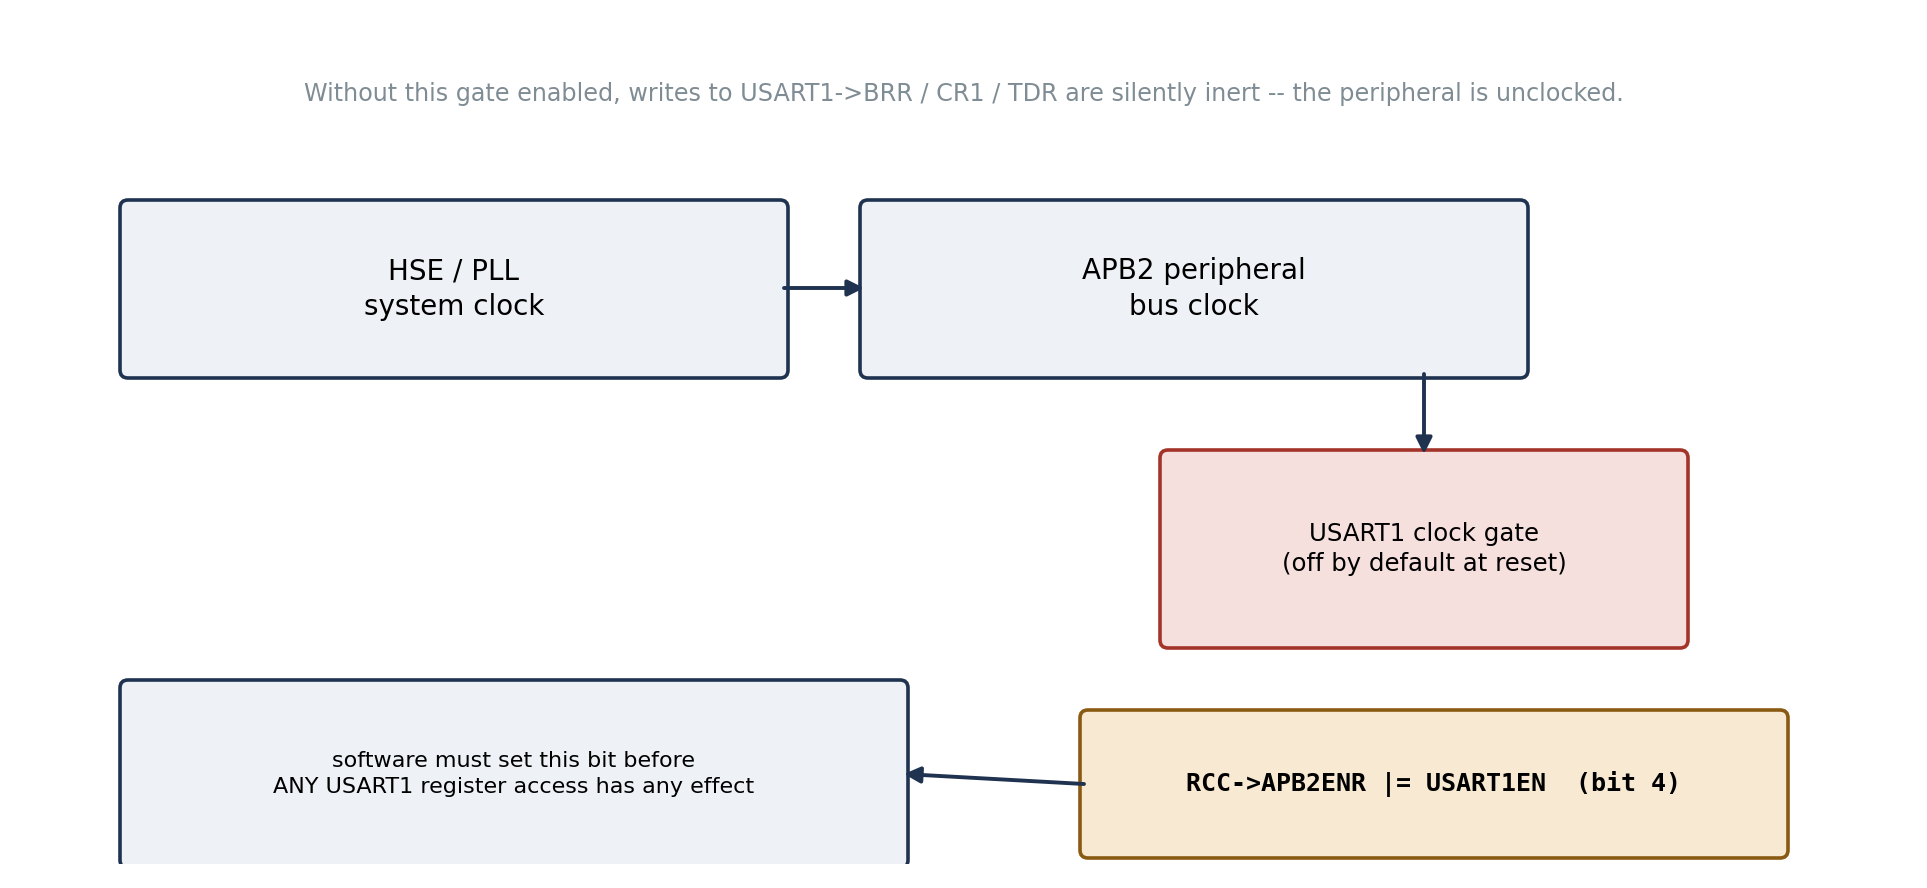
\includegraphics[width=0.98\textwidth]{figures/fig_3_1_clock_gating.png}
\caption{The georeferencing coprocessor pipeline. MAVLink telemetry (100\,Hz) and radar frame-sync (10--50\,Hz) enter from the left; georeferenced WGS84 target coordinates exit to the right.}
\label{fig:3.1}
\end{figure}

\textbf{Stage 1 --- MAVLink DMA Parser:} USART1 RX bytes are moved by DMA1 Stream 0 into a 512-byte circular buffer in AXI SRAM. The parser polls the DMA remaining-count register (or a simulation backdoor) to detect new data, scans for MAVLink v2 magic bytes (\texttt{0xFD}), validates CRC, and dispatches by message ID. Parsed attitude and position data are written to a \texttt{kinematic\_state\_t} struct.

\textbf{Stage 2 --- Hardware Timer Synchronization:} TIM2 (32-bit) free-runs at 1\,MHz (prescaler 239 from 240\,MHz APB1 timer clock). The radar SoC's frame-sync pulse triggers an input capture event that latches \texttt{TIM2\_CNT} into \texttt{TIM2\_CCR1} atomically, providing a microsecond-precise timestamp for the radar sweep.

\textbf{Stage 3 --- Lock-Free Ring Buffer:} A single-producer (parser) / single-consumer (EKF) ring buffer in AXI SRAM holds a rolling window of timestamped kinematic state. DMB barriers ensure correct memory ordering on the Cortex-M7 out-of-order pipeline.

\textbf{Stage 4 --- EKF Fusion:} A 6-state Extended Kalman Filter (state: $[p_n, p_e, p_d, v_n, v_e, v_d]^T$) fuses the drone's inertial state with radar range-azimuth-elevation-doppler measurements. The prediction step uses a constant-velocity model; the update step uses a linearized measurement model with innovation gating. CMSIS-DSP matrix operations run on the Cortex-M7 FPU.

\textbf{Stage 5 --- Coordinate Transform:} Fused target positions in the NED body frame are rotated by the attitude quaternion to ENU, then converted to WGS84 (lat/lon/alt) using the reference position. Doppler velocity is transformed similarly and compensated for drone motion.

\textbf{Stage 6 --- Output Streaming:} Georeferenced targets are packed into binary frames (magic, version, length, sequence, timestamp, target count, per-target records, CRC-32) and streamed over SPI DMA to the ground laptop radio bridge.

\section{System and Memory Architecture}

Figure~\ref{fig:3.2} shows the address-space map. Internal Flash at \texttt{0x08000000} (2\,MB) holds the vector table, code, and read-only data. Internal AXI SRAM at \texttt{0x24000000} (512\,KB) holds the \texttt{.data} and \texttt{.bss} sections, the DMA circular buffer, ring buffer, EKF state matrices, and output frame buffer. External SDRAM at \texttt{0xD0000000} (32\,MB) reached via FMC Bank 2 holds the kinematic history window for extended missions.

\begin{figure}[htbp]
\centering
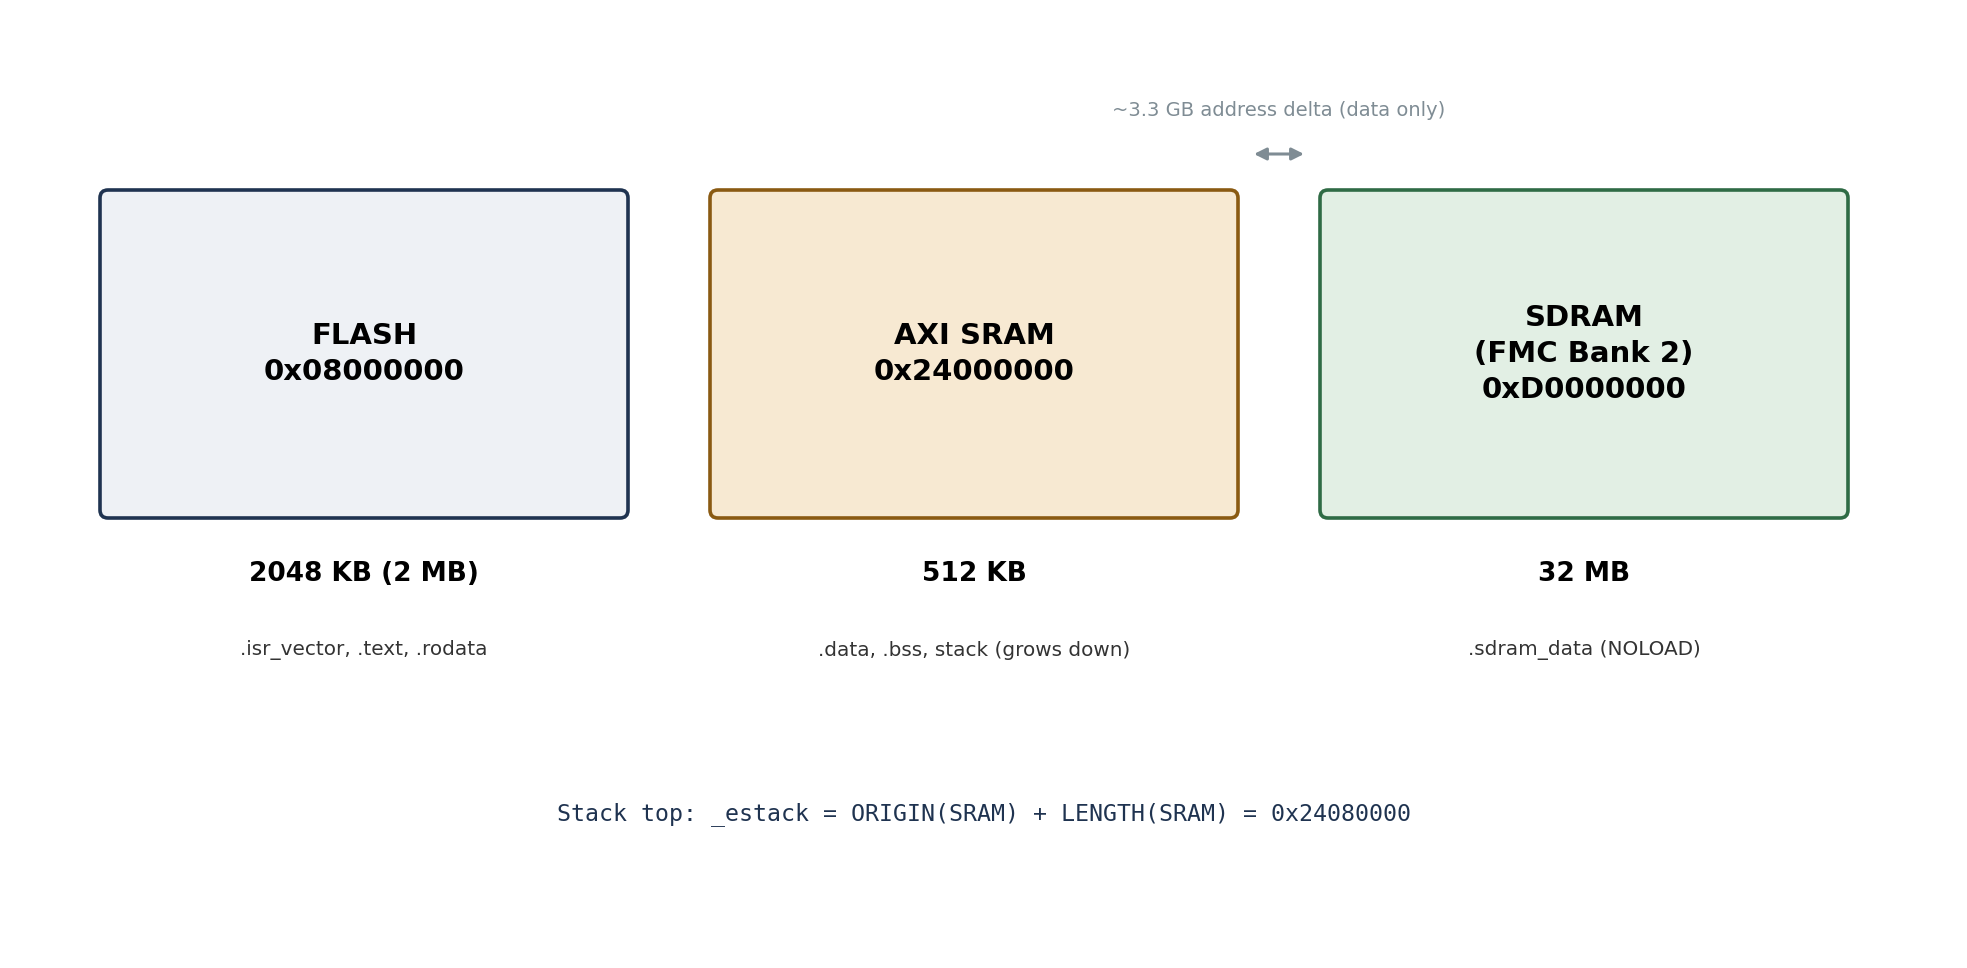
\includegraphics[width=0.95\textwidth]{figures/fig_3_3_memory_map.png}
\caption{System memory map: Flash (code), AXI SRAM (buffers and state), and FMC SDRAM (kinematic history).}
\label{fig:3.2}
\end{figure}

Two architectural details recur as root causes in Chapter~4. First, DMA1 writes directly to physical SRAM, bypassing the CPU's 16\,KB L1 data cache. The CPU reading the same address sees stale cached data unless it explicitly invalidates the cache line via \texttt{SCB\_DCCIMVAC}. Second, the MPU can mark the SDRAM region as Execute-Never (XN); any instruction fetch from SDRAM triggers a MemManage fault unless an MPU region explicitly authorises execution.

\section{Interrupt and Exception Architecture}

The vector table \texttt{g\_pfnVectors[]} has 57 entries (indices 0--56). The interrupts used by this firmware are:

\begin{itemize}
\item \textbf{DMA1 Stream 0 (IRQ 11):} USART1 RX DMA transfer complete --- parser polls, does not use interrupts in circular mode.
\item \textbf{TIM2 (IRQ 28):} Timer overflow for wraparound tracking; input capture is handled in hardware without interrupts.
\item \textbf{EXTI15\_10 (IRQ 40):} Frame-sync input (rising edge) --- sets a flag and latches the timer value.
\end{itemize}

The NVIC priority grouping is left at the default (no sub-priorities). PendSV and SysTick are not used; the firmware runs a single main-loop architecture without an RTOS, eliminating priority-inversion and context-switching defect classes.

\section{Development, Toolchain, and Verification Methodology}

Every pipeline stage is compiled with the GNU Arm Embedded Toolchain, \texttt{arm-none-eabi-gcc}, targeting the Cortex-M7 with hardware floating point (\texttt{-mcpu=cortex-m7 -mthumb -mfloat-abi=hard -mfpu=fpv5-d16}), warnings enabled and optimisation disabled (\texttt{-Wall -Wextra -g3 -O0}). Linking uses a custom \texttt{stm32h753.ld} script, freestanding C runtime (\texttt{--specs=nosys.specs -nostdlib -lc -lnosys -lgcc}), and dead-code elimination.

Table~\ref{tab:3.2} summarises the toolchain. Hardware-in-the-loop stimuli are generated using pymavlink, which produces MAVLink v2 packets with correct CRCs. These packets are injected into the Renode simulation via memory-mapped backdoors in AXI SRAM (addresses \texttt{0x24000010}--\texttt{0x2400001C}), bypassing the unimplemented DMAMUX1 peripheral.

\begin{table}[htbp]
\centering
\caption{Development and verification toolchain.}
\label{tab:3.2}
\begin{tabularx}{\textwidth}{@{}p{3.4cm}Y@{}}
\toprule
\textbf{Stage} & \textbf{Tool / configuration} \\
\midrule
Cross-compilation & \texttt{arm-none-eabi-gcc}, \texttt{-mcpu=cortex-m7 -mthumb -mfloat-abi=hard -mfpu=fpv5-d16 -O0 -g3} \\
Linking & \texttt{arm-none-eabi-ld}, \texttt{stm32h753.ld}, \texttt{--specs=nosys.specs -nostdlib -lc -lnosys -lgcc} \\
Stimuli generation & pymavlink 2.4.49 (Python), MAVLink v2 with correct CRCs \\
Primary verification & Antmicro Renode 1.16.1, scripted via \texttt{simulate.rescript} \\
HIL testing & Real MAVLink packets injected via AXI SRAM backdoors \\
\bottomrule
\end{tabularx}
\end{table}